\documentclass[main.tex]{subfiles}

\begin{document}
\section{Appendix A - User Manual}
\label{user_manual}
\subsection{Launching Thalia}
As Thalia is a web application, it is accessible in a web browser via the url: \urllink{http://thaliabacktest.xyz/}.



\begin{figure}[H]

   \centering

   
\includegraphics[scale=0.8]{08Appendices/081User/081Pictures/thalia_domain.png}

   \caption{Thalia Web}

   \label{thalia_web}

\end{figure}

\subsection{Browsing Thalia}

Navigation within the application can be achieved mainly by the navigation bar, visible on \figurename{\ref{thalia_navbar}}.



\begin{figure}[H]

   \centering

   
\includegraphics[width=\textwidth]{08Appendices/081User/081Pictures/navbar.png}

   \caption{Thalia Navigation Bar}

   \label{thalia_navbar}

\end{figure}



In case Thalia is launched on a different device, such as mobile or in a smaller window, the layout changes to fit the screen. In this case, the navigation bar becomes a so-called "hamburger button" and dropdown menu visible on \figurename{\ref{thalia_navbar_hamburger}}.



\begin{figure}[H]

   \centering

   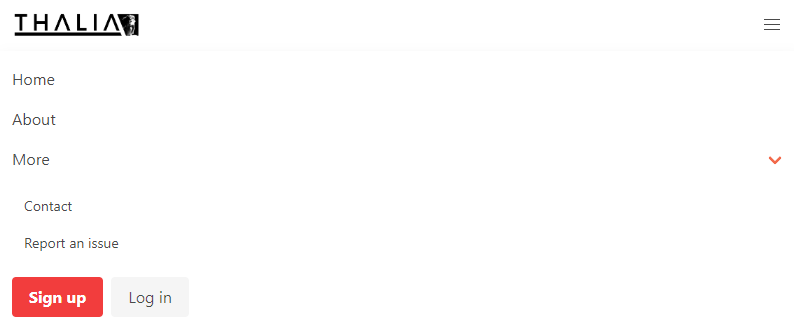
\includegraphics[width=\textwidth]{08Appendices/081User/081Pictures/navbar_hamburger.png}

   \caption{Thalia Navigation Bar - Hamburger}

   \label{thalia_navbar_hamburger}

\end{figure}



For the rest of this manual, we shall assume that the application was launched on a computer, although the layout is identical and intuitive in both cases. 



\subsubsection{Homepage}



By default, the user ends up on the homepage, although some other pages are accessible as well given the correct URL. The Homepage is visible on \figurename{\ref{thalia_home}}.



\begin{figure}[H]

   \centering

   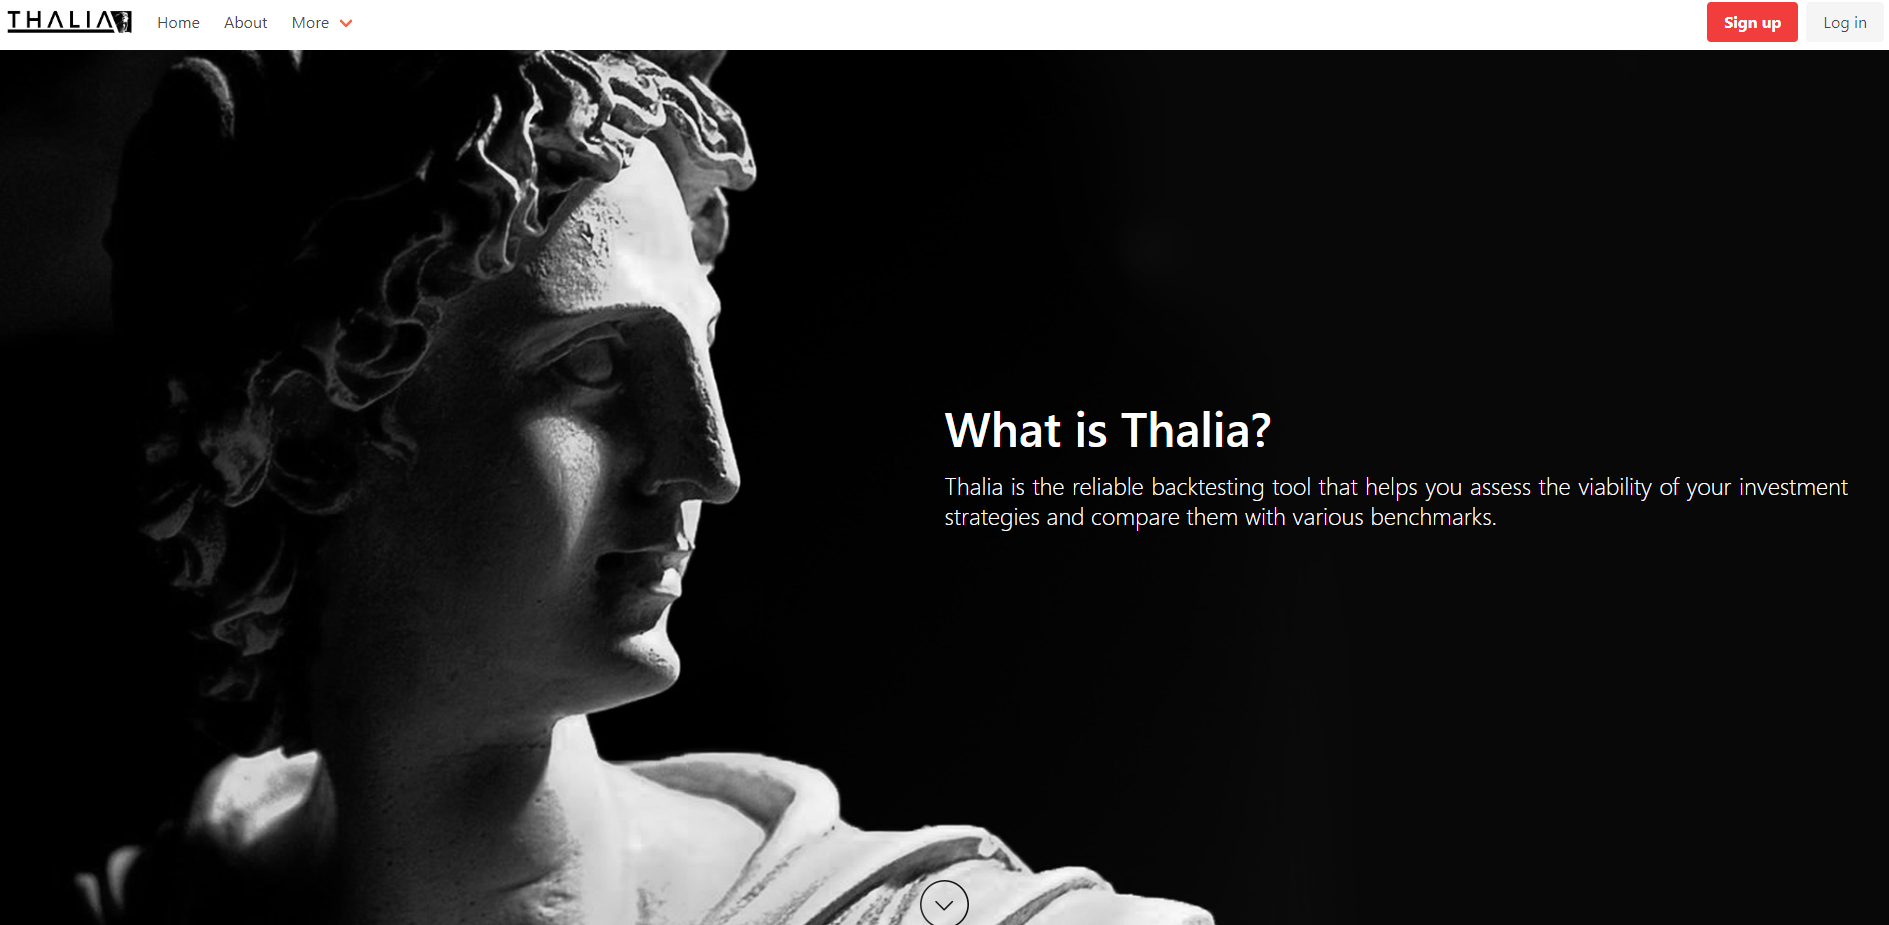
\includegraphics[width=\textwidth]{08Appendices/081User/081Pictures/homepage.png}

   \caption{Thalia Homepage (source: http://thaliabacktest.xyz/)}

   \label{thalia_home}

\end{figure}



The purpose of the homepage is to give a cover to our application. As users arrive at the homepage, they are greeted with a short description of what our software actually is.

As we do not wish to have users jumping blindly into the process of portfolio analysis, following that we provide some basic information on the backtesting process. A link at the end of the description then leads to the about page, where users can read more on the topic.



Scrolling further down the user may encounter a small register form, or in case the user is logged in, our tweets and social media links.



\begin{figure}[H]

   \centering

   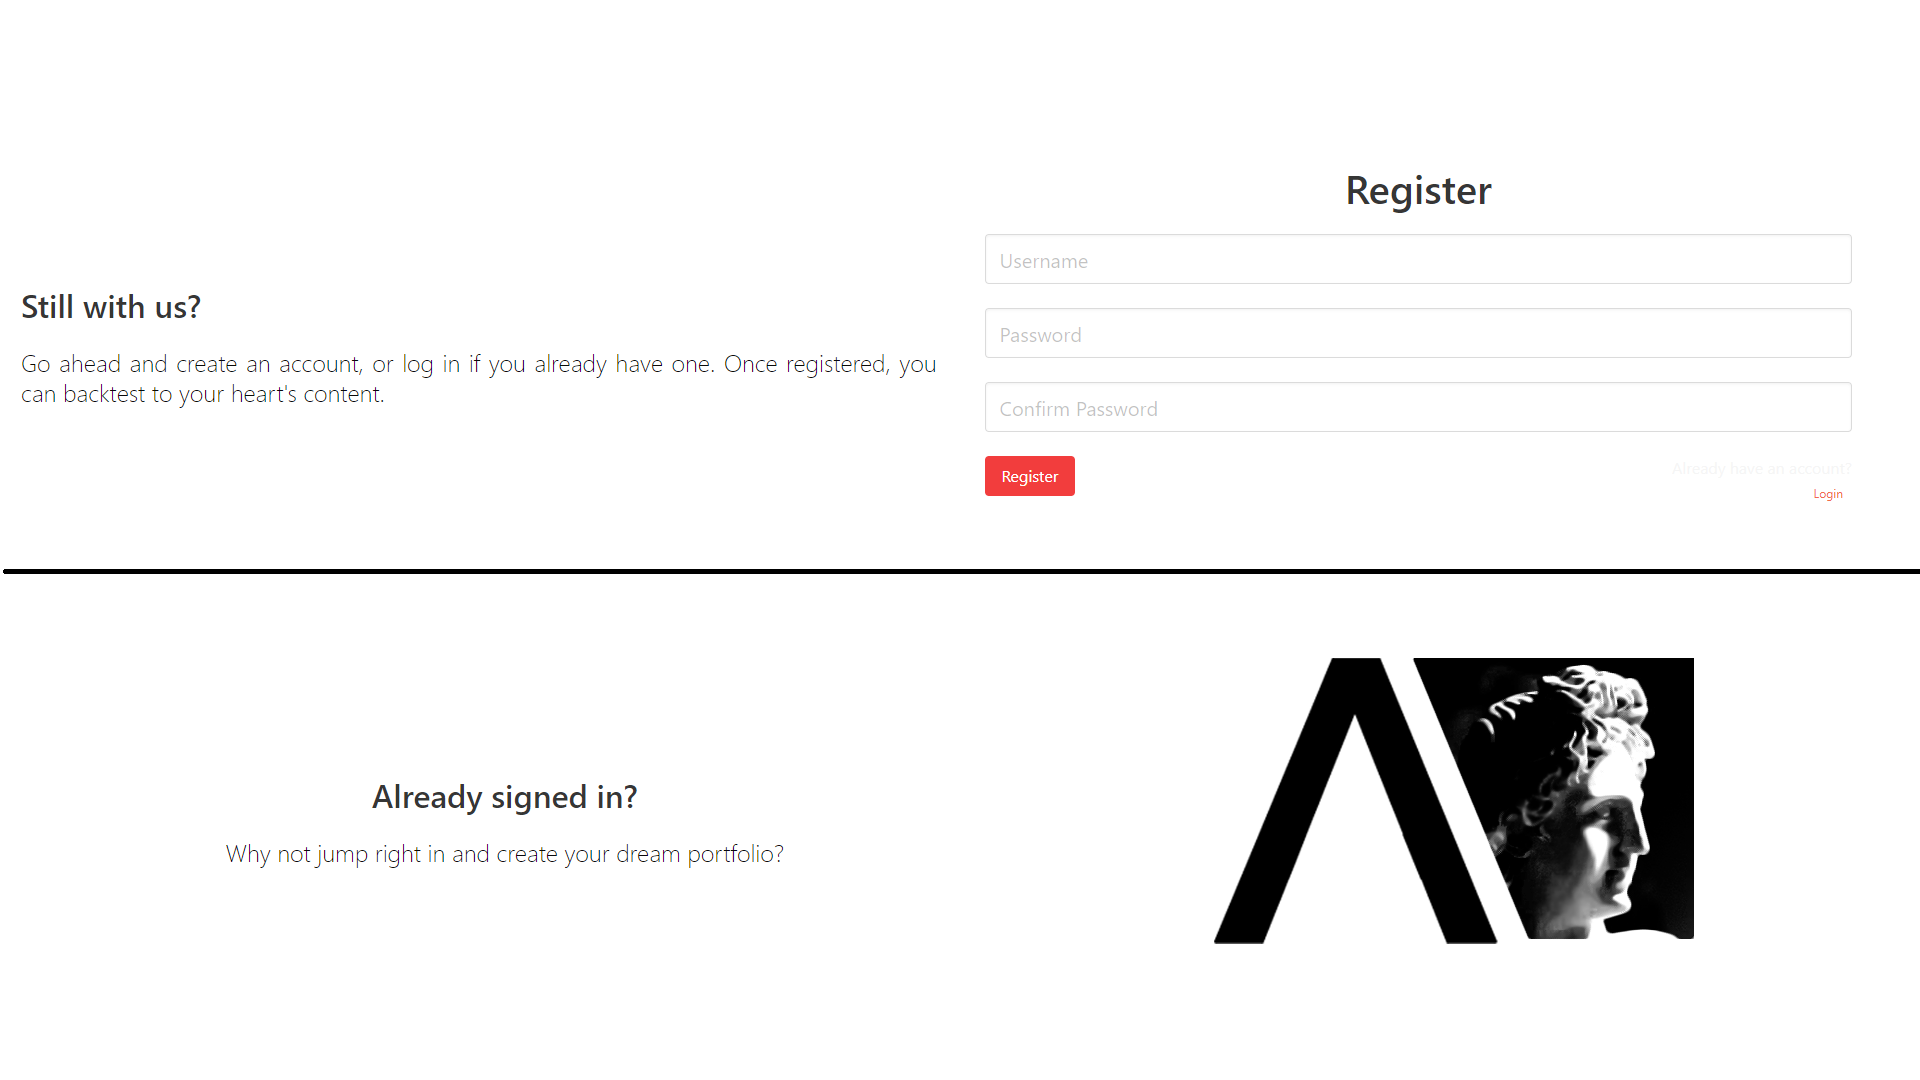
\includegraphics[width=\textwidth]{08Appendices/081User/081Pictures/homepage_bottom.png}

   \caption{Thalia Homepage 2 - Top: User not logged in; Bottom: User recognised}

   \label{thalia_home_bottom}

\end{figure}



\subsubsection{About Page}



The about page of our application is to provide a more detailed description of the problem domain and is available at \urllink{http://thaliabacktest.xyz/about/}.

The user can arrive at this page either by directly typing in the URL, clicking on the learn more option on the Homepage, or by navigating here using the navigation bar.



Our About Page looks as follows:



\begin{figure}[H]

   \centering

   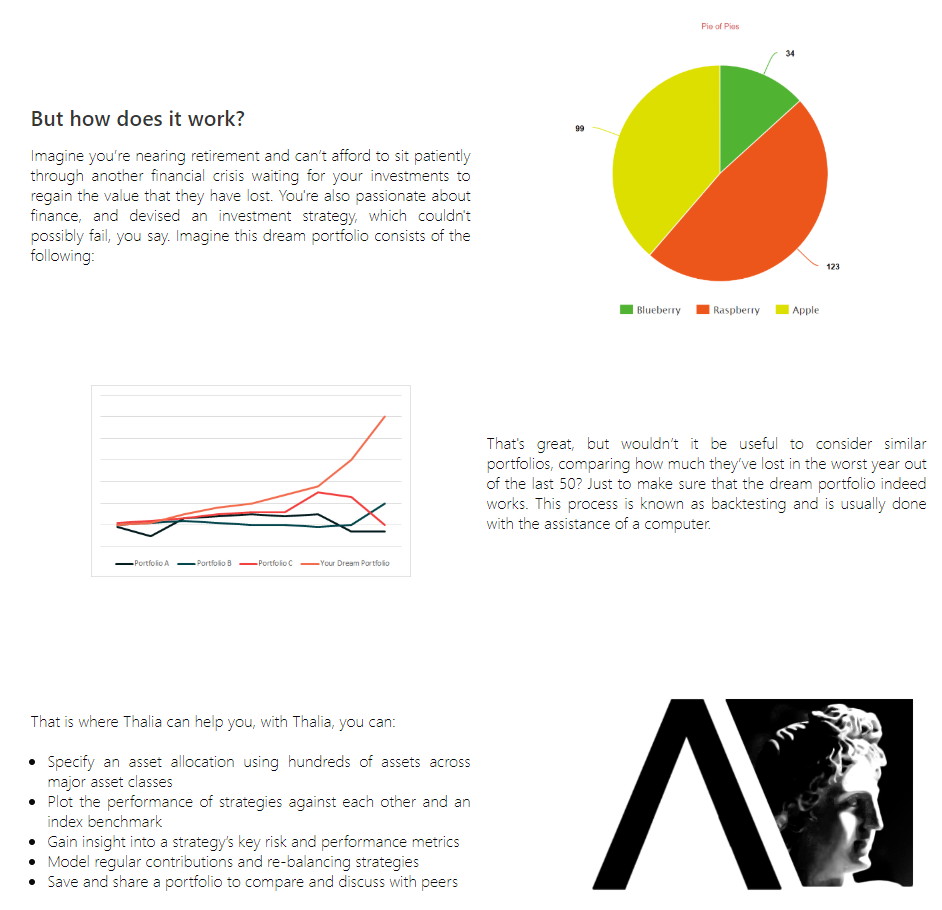
\includegraphics[width=\textwidth]{08Appendices/081User/081Pictures/about.png}

   \caption{Thalia About Page (source: http://thaliabacktest.xyz/about/)}

   \label{thalia_about}

\end{figure}



\subsubsection{Log In and Sign Up Pages}

In case the User is not yet logged in, links for the Log In and Sign Up pages are visible on the navigation bar as seen on \figurename{\ref{thalia_navbar}} or \figurename{\ref{thalia_navbar_hamburger}}. In addition, they are directly available at \urllink{http://thaliabacktest.xyz/login/} and \urllink{http://thaliabacktest.xyz/register/}.

Both of these forms are quite common, with the login requiring:



\begin{itemize}

    \item Username

    \item Password

    \item Remember me: Optional

\end{itemize}



And for signing up, the fields are:



\begin{itemize}

    \item Username

    \item Password: Minimum eight characters,at least one letter, one number and one special character

    \item Confirm Password: Same as Password

\end{itemize}



As standard, the registration fails when the user enters different values to the Password and Confirm Password fields. In this case, the user is prompted to try again.



\begin{figure}[H]

   \centering

   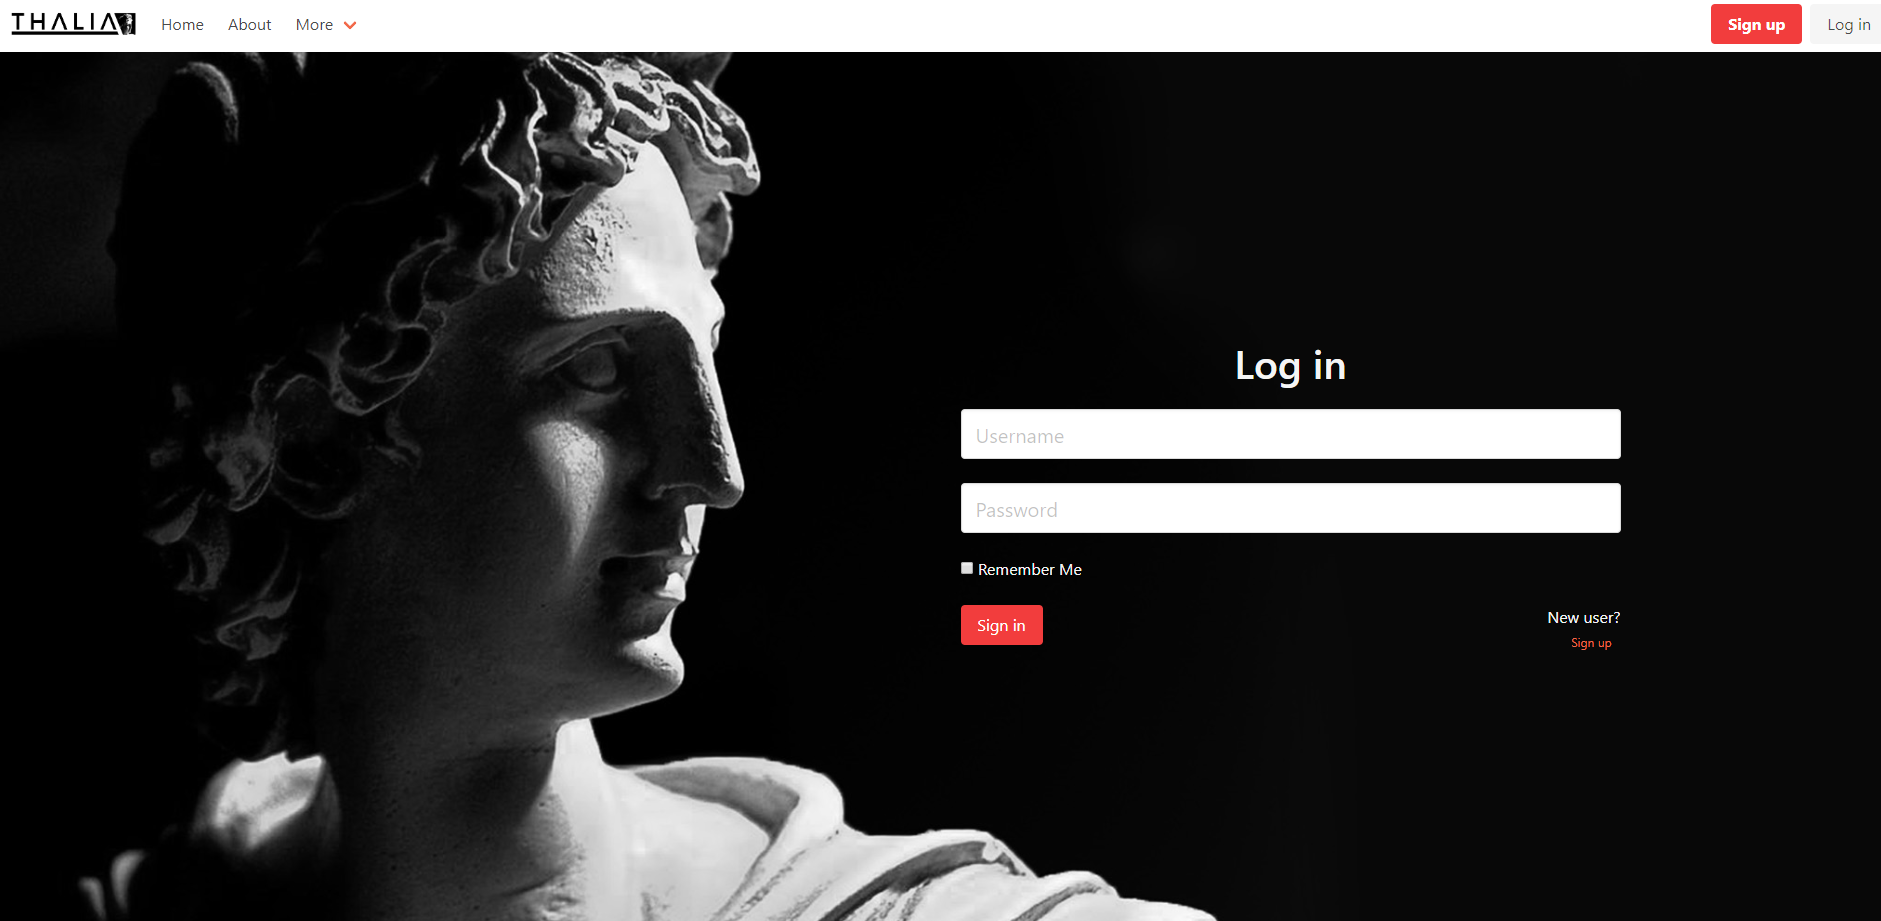
\includegraphics[width=\textwidth]{08Appendices/081User/081Pictures/login.png}

   \caption{Thalia Log In Page (source: http://thaliabacktest.xyz/login/)}

   \label{thalia_login}

\end{figure}



In case the user is already logged in and attempts to access these pages, he or she gets redirected to the homepage. In addition, the navigation bar changes, allowing to log out as visible on \figurename{\ref{thalia_issues}}.

Opting to log out the user finds themselves at the homepage.



\subsubsection{Contact Us Page}



The Report Issues Page is available at \urllink{http://thaliabacktest.xyz/contact/} or via opening the dropdown menu on the navigation bar and clicking the link. This short form is for users to provide feedback, report possible issues or request features.



\begin{figure}[H]

   \centering

   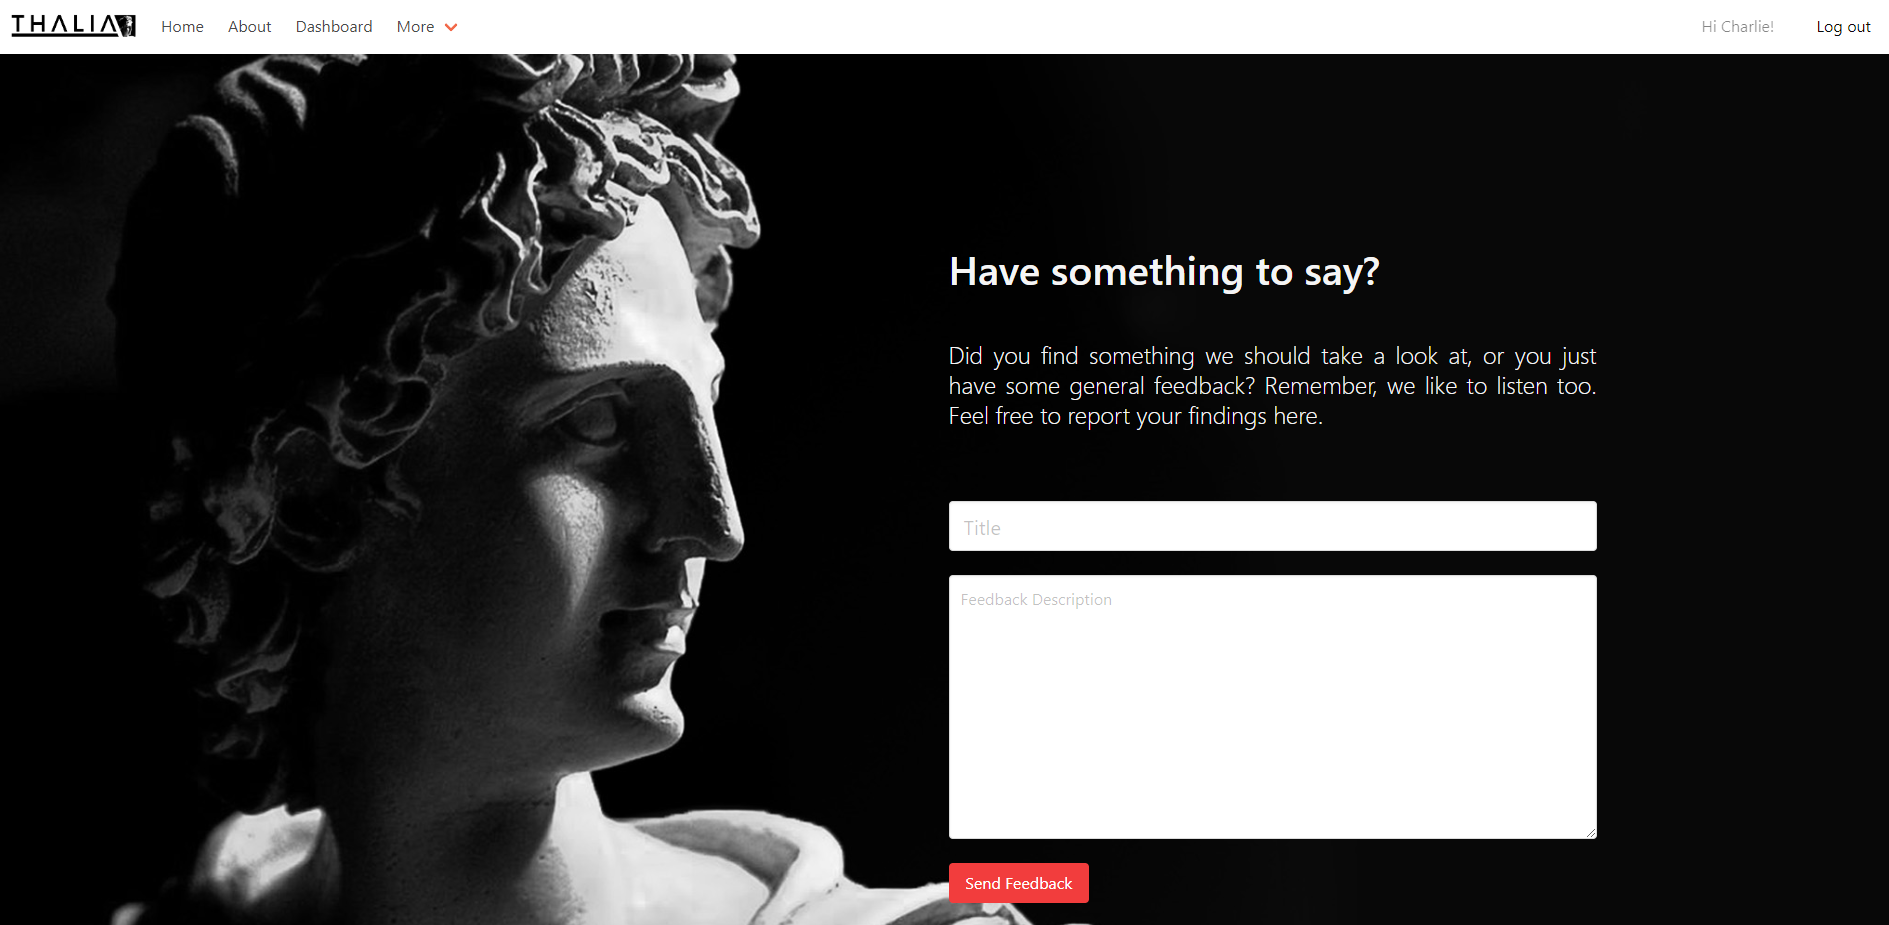
\includegraphics[width=\textwidth]{08Appendices/081User/081Pictures/issues.png}

   \caption{Thalia Report Issues Page (source: http://thaliabacktest.xyz/contact/)}

   \label{thalia_issues}

\end{figure}



\subsubsection{About Us Page}

We also wanted to take pride in our project and sign are work, following \cite{pragmaticprog_sign}. This simple page is dedicated to the team behind Thalia.



\subsubsection{My Portfolios Page}

The My Portfolios Page is only accessible for authenticated users. Here the user may view their saved portfolios with their asset allocations, and load them by clicking the corresponding boxes. Doing so the user will find themselves on the Dashboard. 

\subsection{Running a Backtest}

To run a backtest, first the user must be authenticated. After a succesful registration and login process the user can head to the Dashboard

\subsubsection{Dashboard}

The Dashboard, our main application, is available only if the user is logged in at \urllink{http://thaliabacktest.xyz/dashboard/} or via the link on the navigation bar.

This web page is divided into tabs, which are:

\begin{itemize}
    \item Ticker Selector
    \item Summary
    \item Metrics
    \item Returns 
    \item Drawdowns
    \item Assets
    \item Overfitting
\end{itemize}

At first, only the Ticker Selector Page is accessible for the user. 

This is because the following tabs show only the output of backtesting a or multiple portfolios, and as a consequence are, for the time being, empty.

\begin{figure}[H]

   \centering

   
\includegraphics[width=\textwidth]{08Appendices/081User/081Pictures/disabled_tabs.png}

   \caption{Thalia Dashboard - Disabled Tabs}

   \label{thalia_disabled_tabs}

\end{figure}

Let us now consider each tab individually. 



\subsubsection{Ticker Selector}



Here the user is required to input their backtesting strategy. As Thalia supports testing multiple portfolios at once (up to 5 currently) there are input fields that are portfolio specific and that are not. The latter consists only of:



\begin{itemize}

    \item Start Date: The day the investment is made.

    \item End Date: The last day of the investment, defaulted to the present date.

    \item Initial Amount: Initial balance, the default currency is dollars.

\end{itemize}



The first two of these are standard date-selectors, but also allow for typing the date directly. Next, the user enters the data specific to the current strategy.



\begin{itemize}

    \item Portfolio Name: Defaulted to Portfolio 1, Portfolio 2, etc. 

    \item Contribution Amount: The amount that should be regularly invested in the portfolio.

    \item Contribution Frequency: Specify how regularly should these contributions be.

    \item Rebalancing Frequency: Specify how often rebalancing should happen. 

    \item Asset Allocations: Discussed below.

\end{itemize}



The last one is the most crucial information in a strategy. First, the user selects the desired asset from the dropdown menu. The menu item also allows for typing in order to find an asset faster. The selected item is then added to the table below.



\begin{figure}[H]

   \centering

   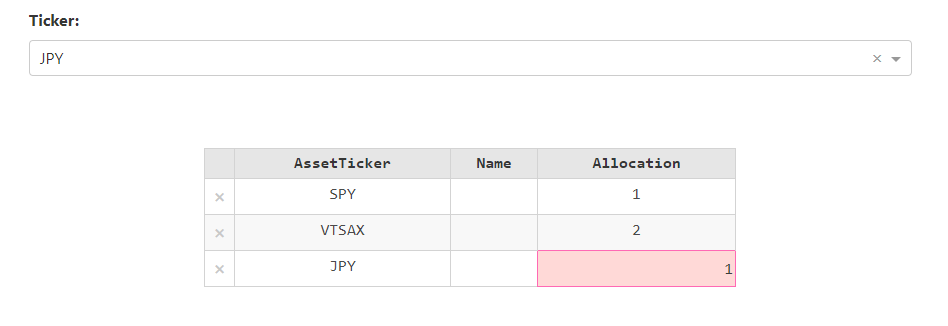
\includegraphics[width=\textwidth]{08Appendices/081User/081Pictures/table.png}

   \caption{Thalia Dashboard - Asset Table (source: http://thaliabacktest.xyz/dashboard/)}

   \label{thalia_table}

\end{figure}


The user then specifies the proportion of the investment, this is required to be a numeric value, representing the relative weight of the asset. For example, given Asset A with relative weight 1, and Asset B with relative weight 2, then they 33\% of the investment comes from Asset A and 66\% from Asset B.

In case the user is content with the portfolio, they can either add another strategy via the "Add Portfolio" button or click "Submit" to see the results. In case the user has already entered the maximum number of portfolios, i.e. 5, the button is disabled and the only possibility is to submit.

If the user has not entered some required data, such as an initial amount, or selected at least one asset, a warning message is shown, telling them to complete the form correctly. Note that this also happens when the user selects a time frame shorter than a year, as many of our metrics do not make sense for investments for such short periods of time.

In many cases the user may want to compare their portfolio to a benchmark, that is to a small set of predetermined portfolios. These can be selected from the "Lazy" dropdown at each portfolio, which then populates the table with the desired proportions.

Alternatively, the user may want to test an allocation on a price data only they have. Given that the user has the data in the format of a CSV file, this can be done by simple drag and drop to the corresponding field. 


\begin{figure}[H]
   \centering
   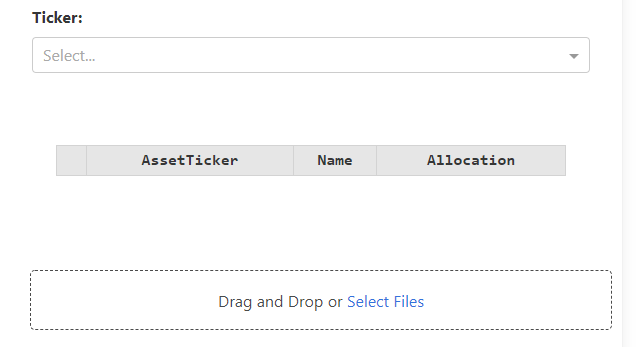
\includegraphics[scale=0.6]{08Appendices/081User/081Pictures/user_csv.png}
   \caption{User Uploaded Data Field}
\end{figure}

\subsection{Viewing the Results}

The result of the backtesting process is divided between the remaining tabs of the dashboard. Let us now discuss what each of them can tell to the user.

\subsubsection{Summary}


If all required fields are populated, the user is taken to the summary tab. This as well as all other tabs are now unlocked. At this point the user is shown one of the key components of our application, i.e. the portfolio growth graph. Thanks to Dash this, and all other graphs are fully interactive. The user may zoom in on selected areas, hover over desired data points, save plot as image, etc.



\begin{figure}[H]

   \centering

   
\includegraphics[width=\textwidth]{08Appendices/081User/081Pictures/dash_funcionalities.png}

   \caption{Dash Functionalities}

   \label{dash_functionalities}

\end{figure}



The plot seen at the top of \figurename{\ref{summary}} shows the total return of each portfolio. Users will typically use this graph for comparison. In addition, for each portfolio the user has given as input, the following is shown:

\begin{itemize}

    \item Selected Key Metrics: Final Balance, Best Year, Worst Year, etc.

    \item Pie Chart: Proportion of each asset.

    \item Bar Chart: Shows how the total return changed over the years relative to the last.

\end{itemize}

\begin{figure}[H]

   \centering

   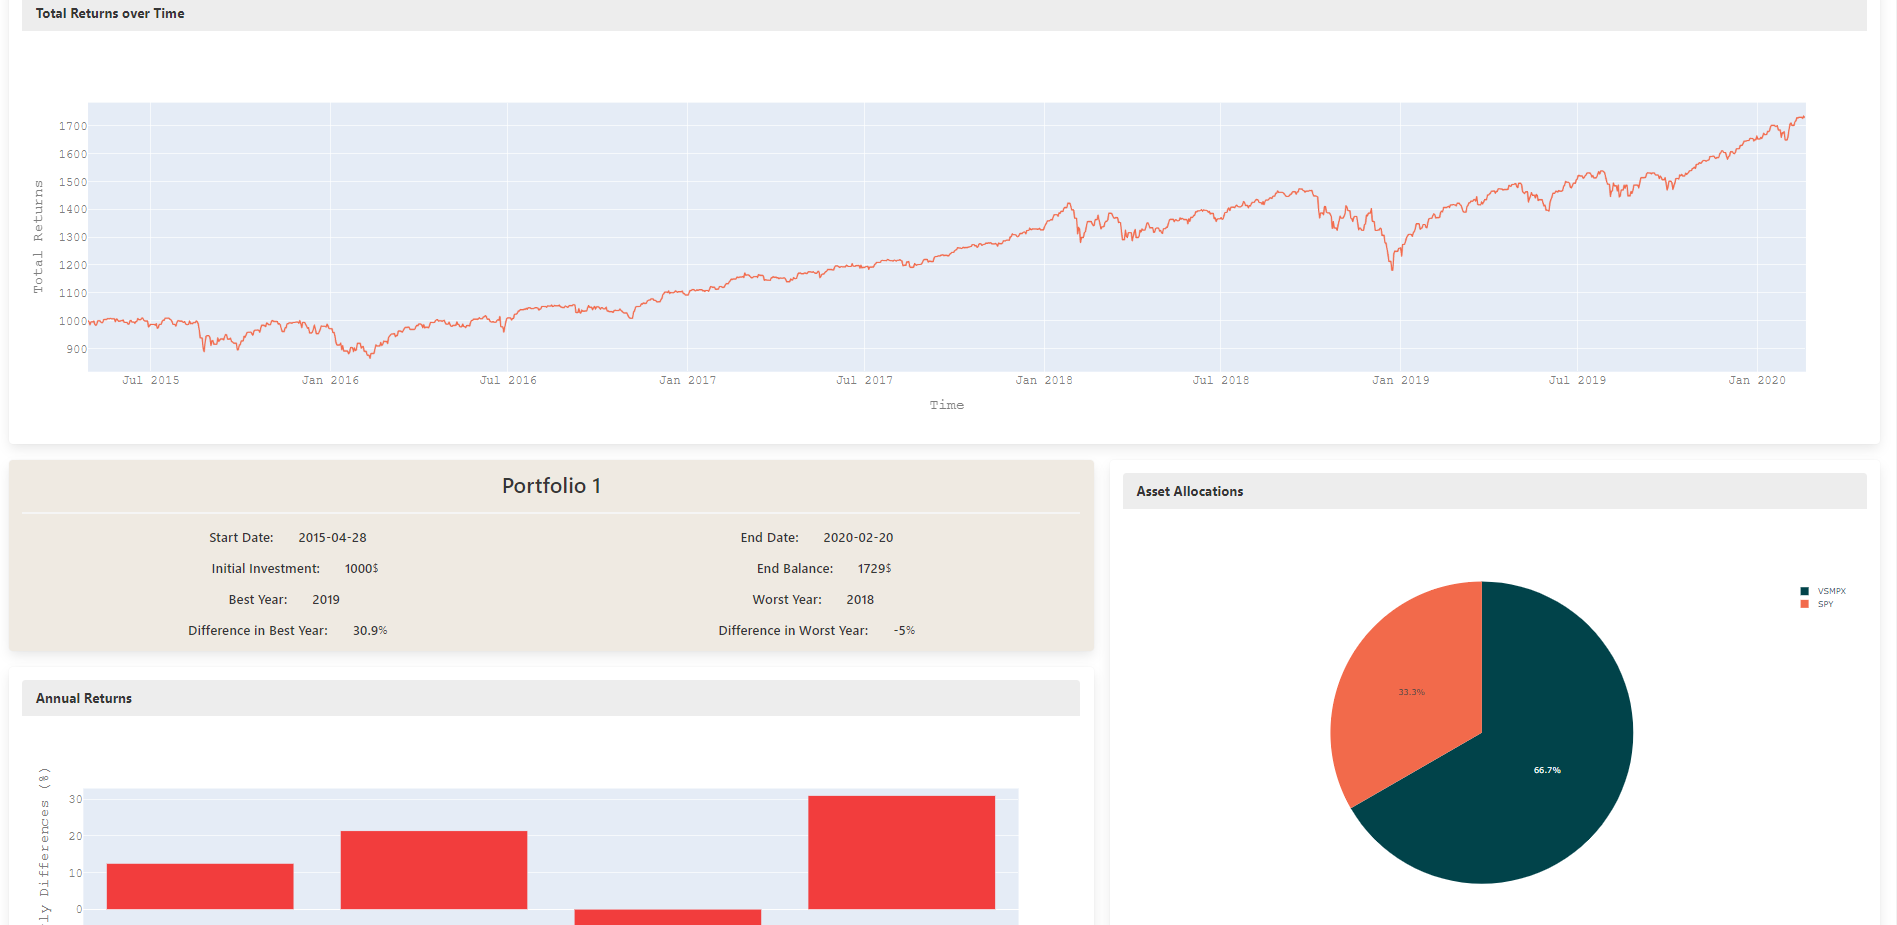
\includegraphics[width=\textwidth]{08Appendices/081User/081Pictures/summary.png}

   \caption{Summary Tab (source: http://thaliabacktest.xyz/dashboard/)}

   \label{summary}

\end{figure}



It is also important to note that in some cases there is no data for a given asset. For example, there is no price data for cryptocurrencies before the 2000s in general as they did not yet exist. In the edge cases, where the portfolio is made up entirely of these assets, the strategy may not be valid in a given investment period. 



If there is only one portfolio given as input and affected by the above, the data fits around the tighter time frame and behaves as if that was the actual investment period. In the case where the user provides more than one investment strategies with different time frames, we provide output where price data is available. As for example on the following graph:



\begin{figure}[H]

   \centering

   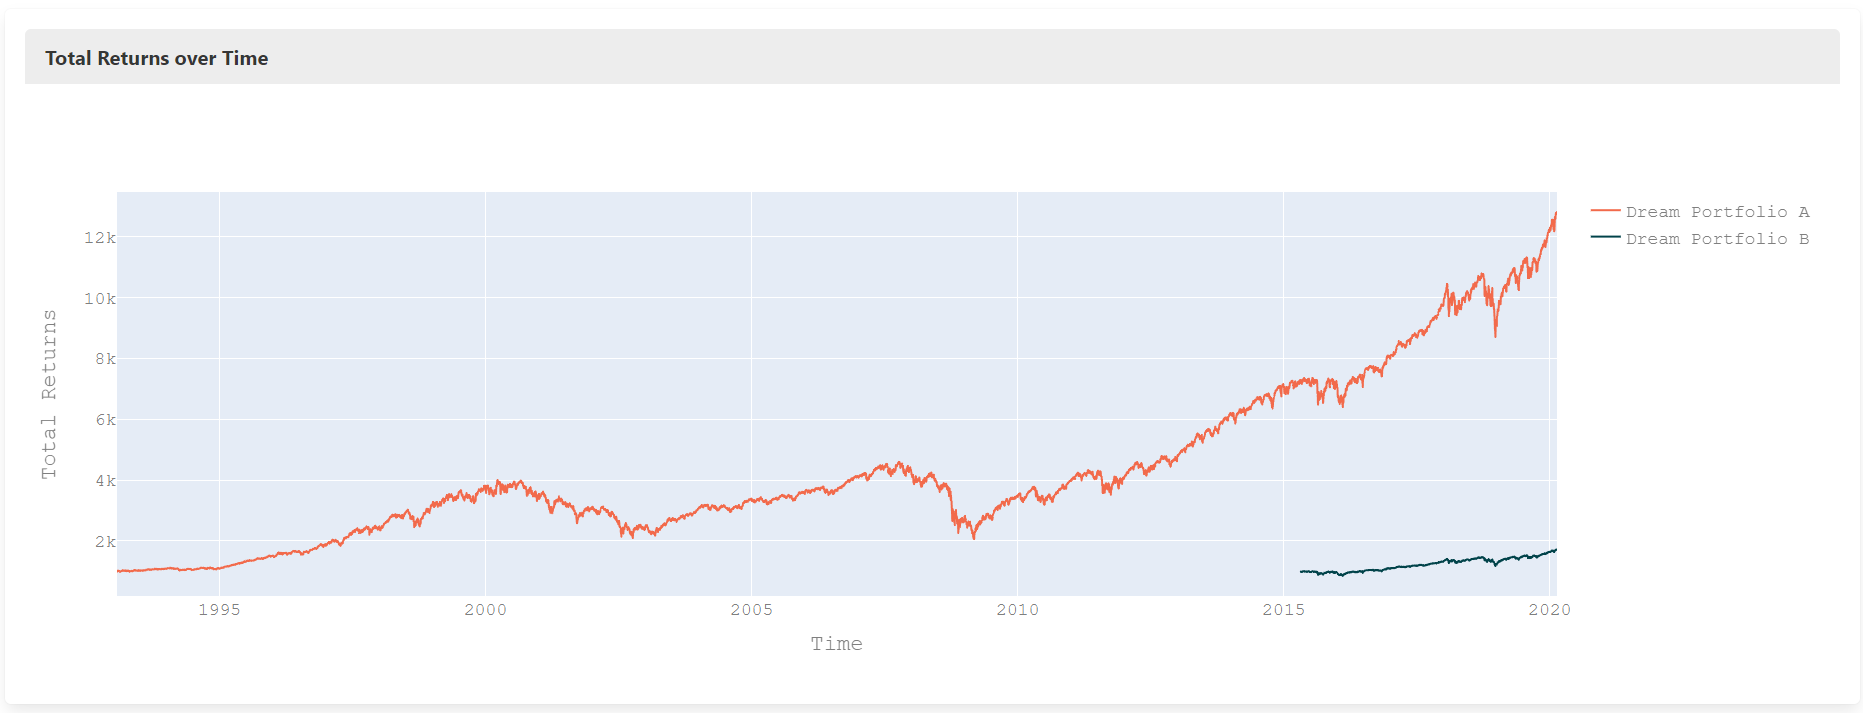
\includegraphics[width=\textwidth]{08Appendices/081User/081Pictures/differences.png}

   \caption{Different Time Frames per Portfolio (source: http://thaliabacktest.xyz/dashboard/)}

\end{figure}



\subsubsection{Metrics}



The Metrics Tab Shows a simple table of key metrics per portfolio. This allows for a quick comparison of strategies. Albeit this page does not show much more data than the previous one, it could easily be expanded later. In case the table gets bigger than the browser window, a horizontal scroller can be used for viewing the rest. 



\begin{figure}[H]

   \centering

   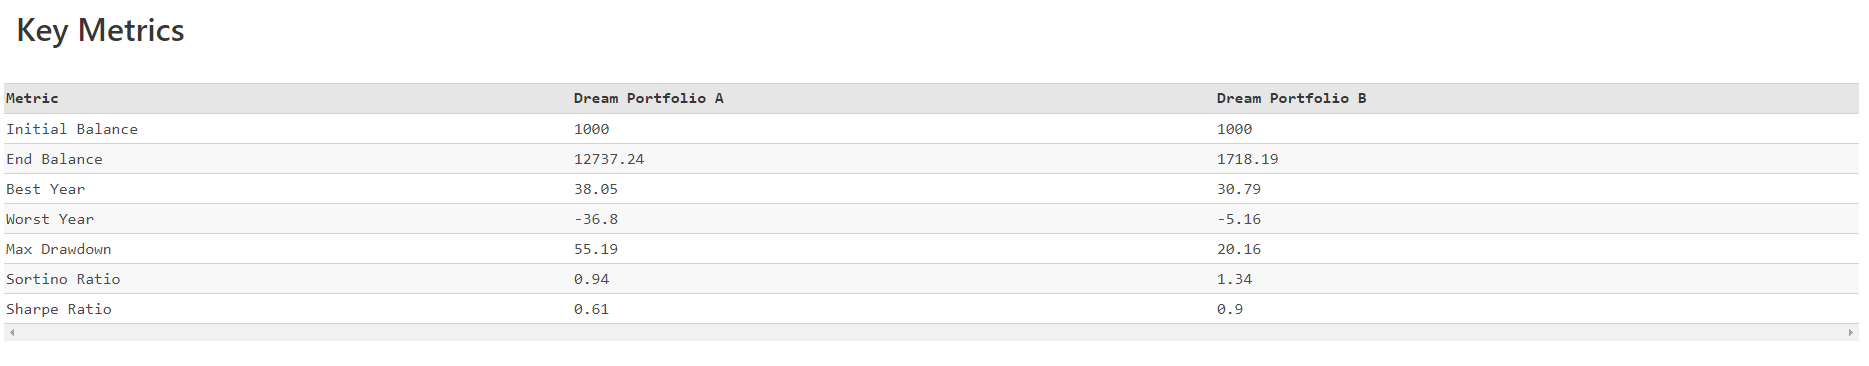
\includegraphics[width=\textwidth]{08Appendices/081User/081Pictures/metrics.png}

   \caption{Metrics Tab (source: http://thaliabacktest.xyz/dashboard/)}

   \label{metrics}

\end{figure}



\subsubsection{Returns}



The Returns Tab allows the user to compare the annual income of each portfolio. It consists of a bar chart similar to the one on the Summary Tab, and a table similar to the one on the Metrics Tab. The graph can be seen on \figurename{\ref{returns}}.



\begin{figure}[H]

   \centering

   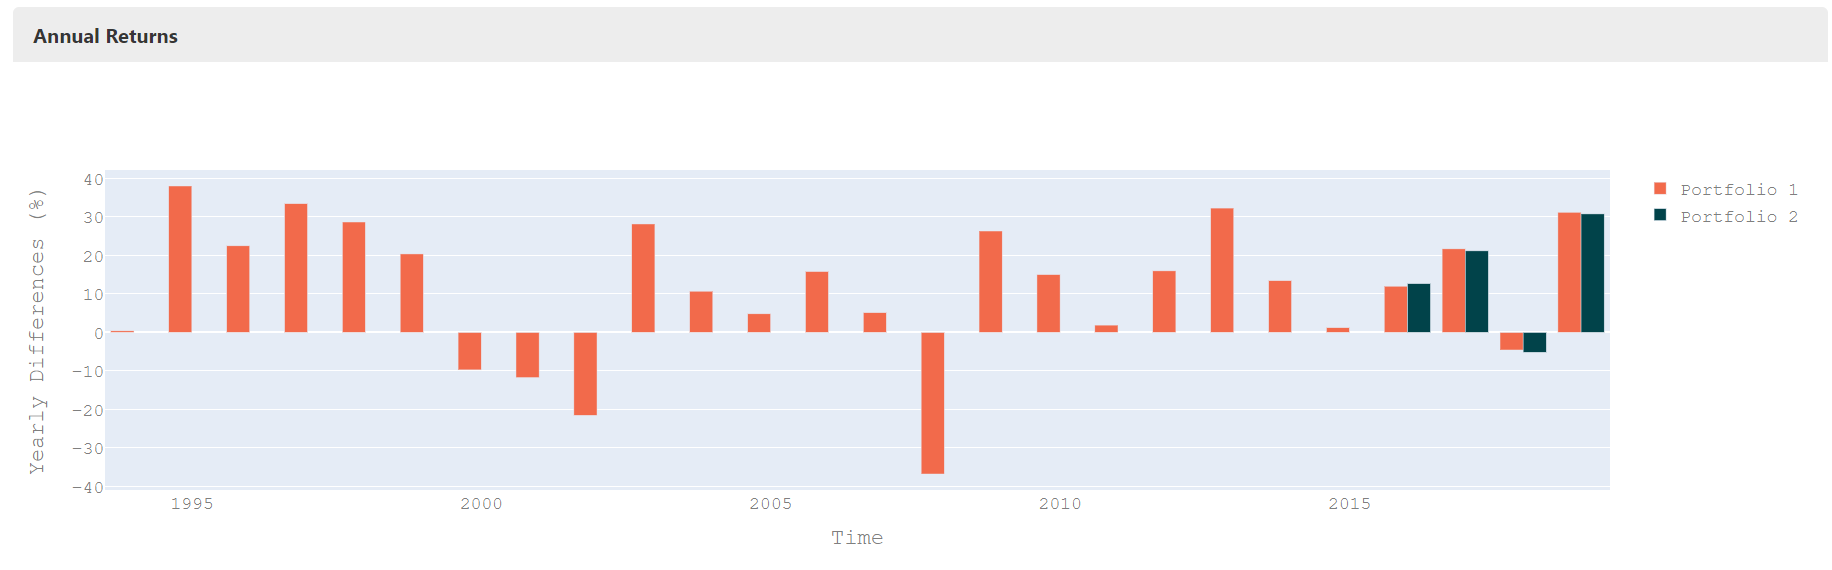
\includegraphics[width=\textwidth]{08Appendices/081User/081Pictures/returns_graph.png}

   \caption{Metrics Tab (source: http://thaliabacktest.xyz/dashboard/)}

   \label{returns}

\end{figure}



It may happen that one of the portfolios was not available at certain times and there is no data for their assets. In these cases, we do not show any values. 



\subsubsection{Drawdowns}



The Drawdowns Tab shows declines during the investment periods. This is shown both on a graph comparing each portfolio visible on \figurename{\ref{drawdowns_graph}}.



\begin{figure}[H]

   \centering

   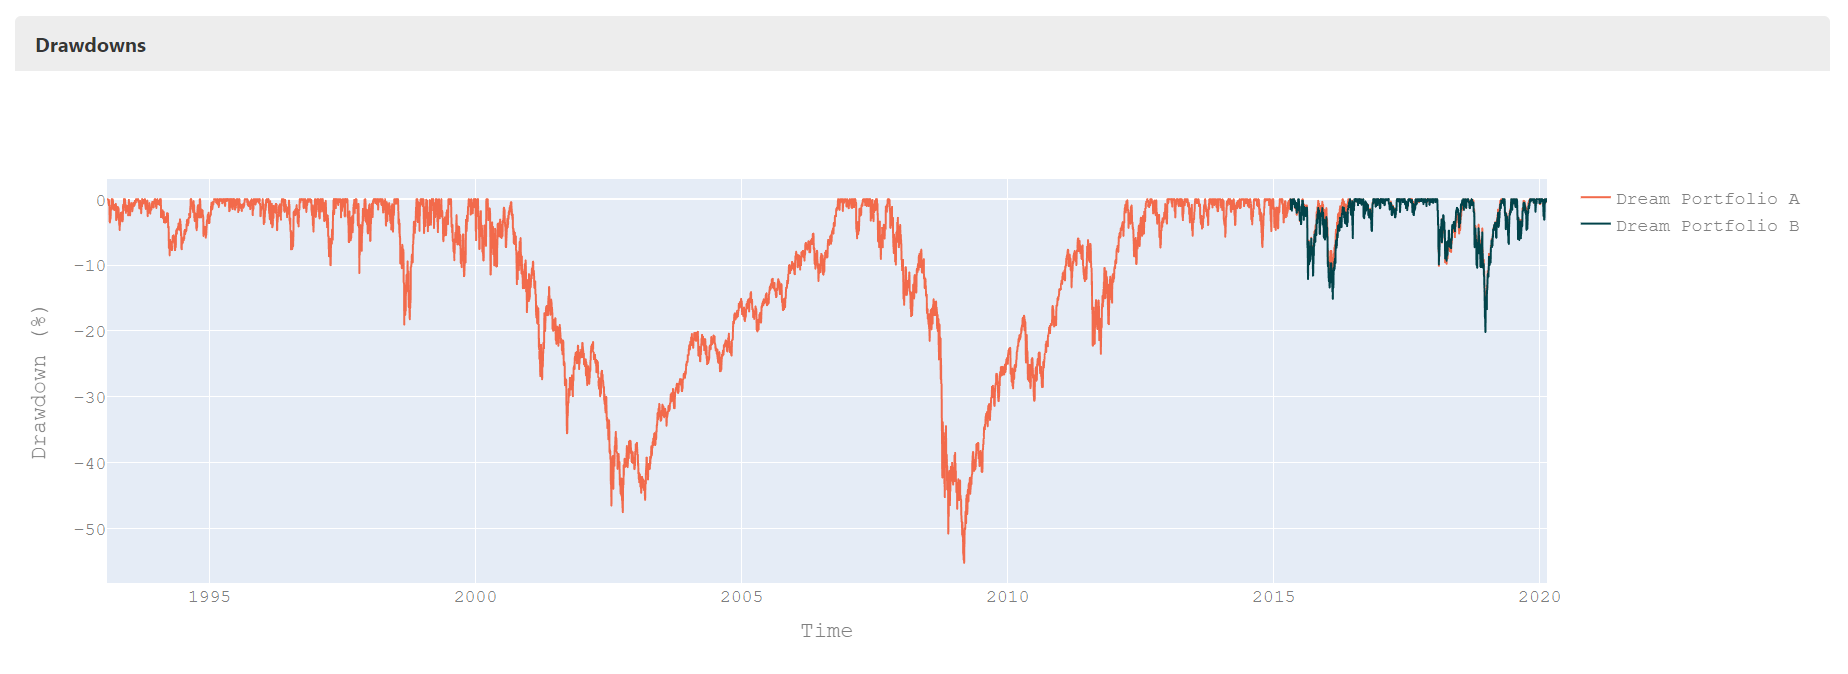
\includegraphics[width=\textwidth]{08Appendices/081User/081Pictures/drawdowns_graph.png}

   \caption{Drawdowns Tab - Graph (source: http://thaliabacktest.xyz/dashboard/)}

   \label{drawdowns_graph}

\end{figure}



For a deeper insight, a table of the top drawdowns is generated for each portfolio. By default, this will be the top 10, or less in case the portfolio does not have 10 drawdown periods. 



\begin{figure}[H]

   \centering

   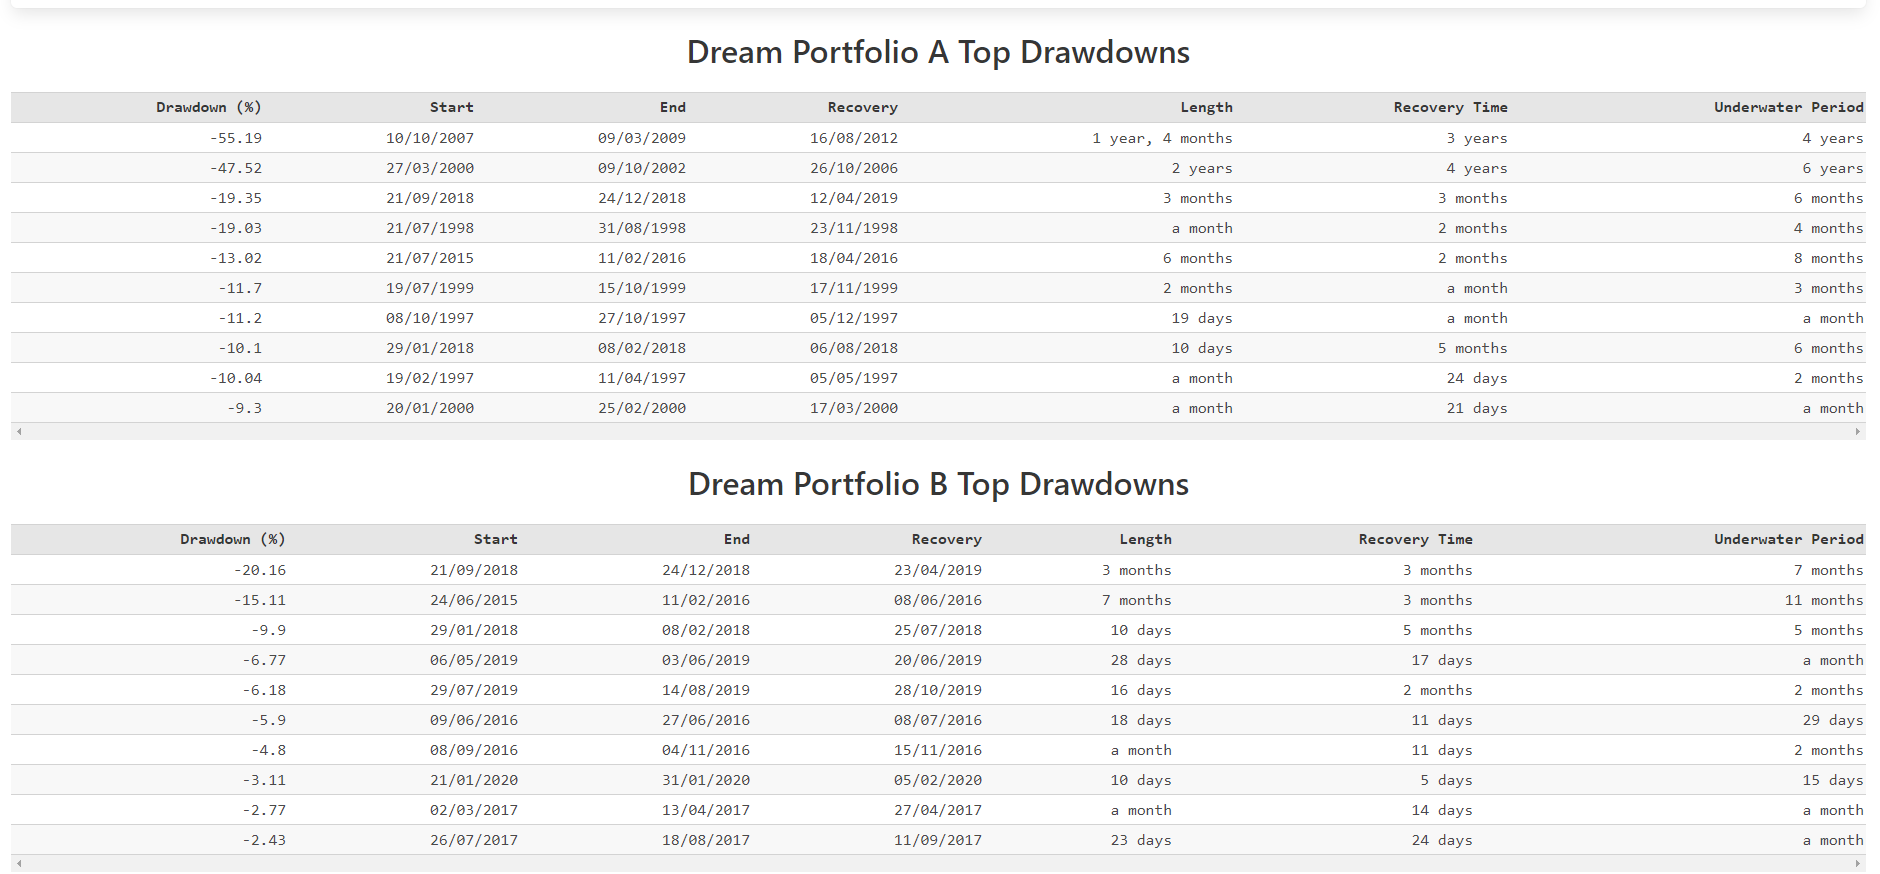
\includegraphics[width=\textwidth]{08Appendices/081User/081Pictures/drawdowns_tables.png}

   \caption{Drawdowns Tab - Tables (source: http://thaliabacktest.xyz/dashboard/)}

   \label{drawdowns_table}

\end{figure}



\subsubsection{Assets}

Here the user may encounter a pie chart similar to the one on the summary tab. Here however, the pie chart shows the proportions of the asset classes and not the assets allocations. This is crucial information for the user as it can show how diverse their portfolio is.

\begin{figure}[H]
   \centering
   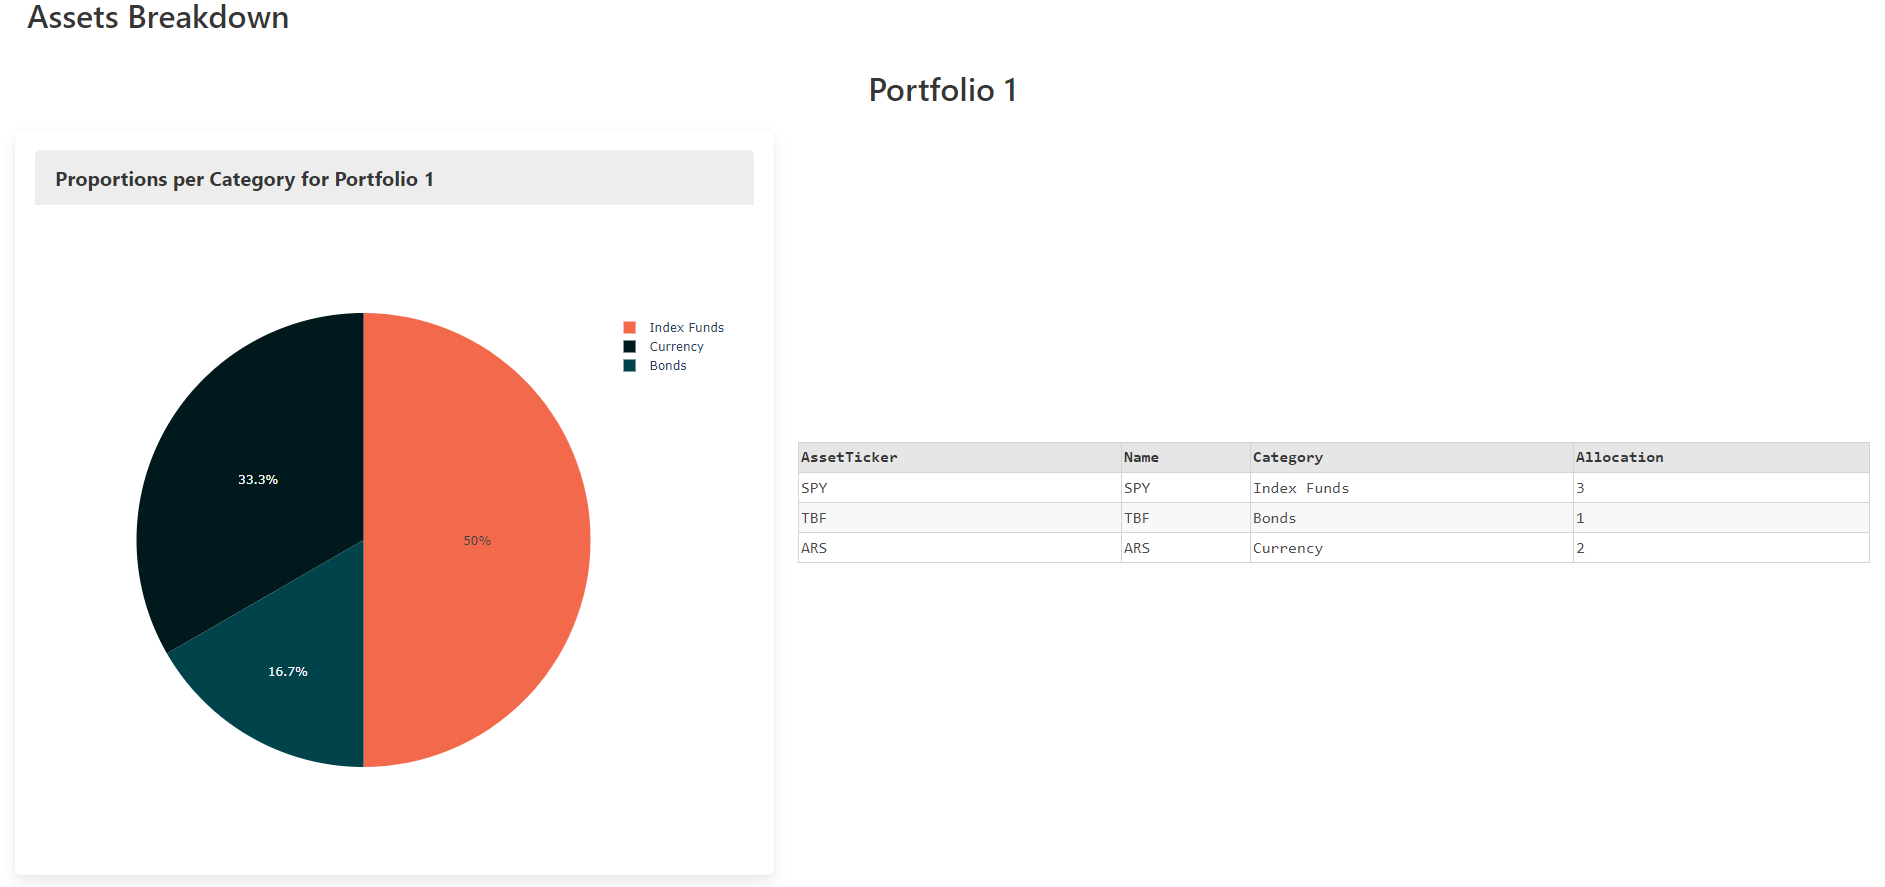
\includegraphics[width=\textwidth]{08Appendices/081User/081Pictures/assets.png}
   \caption{Assets Tab (source: http://thaliabacktest.xyz/dashboard/)}
   \label{assets_tab}
\end{figure}

\subsubsection{Overfitting}

Our last results tab encompasses a relatively complex feature, which is overfitting. Here the user may test if any of their portfolios has been tweaked to fit to the trends a little too much, making it an unrealistic investment. In case the user decides to run the overfitting test and it fails to detect an overfitting tendency, it shows:

\begin{figure}[H]
   \centering
   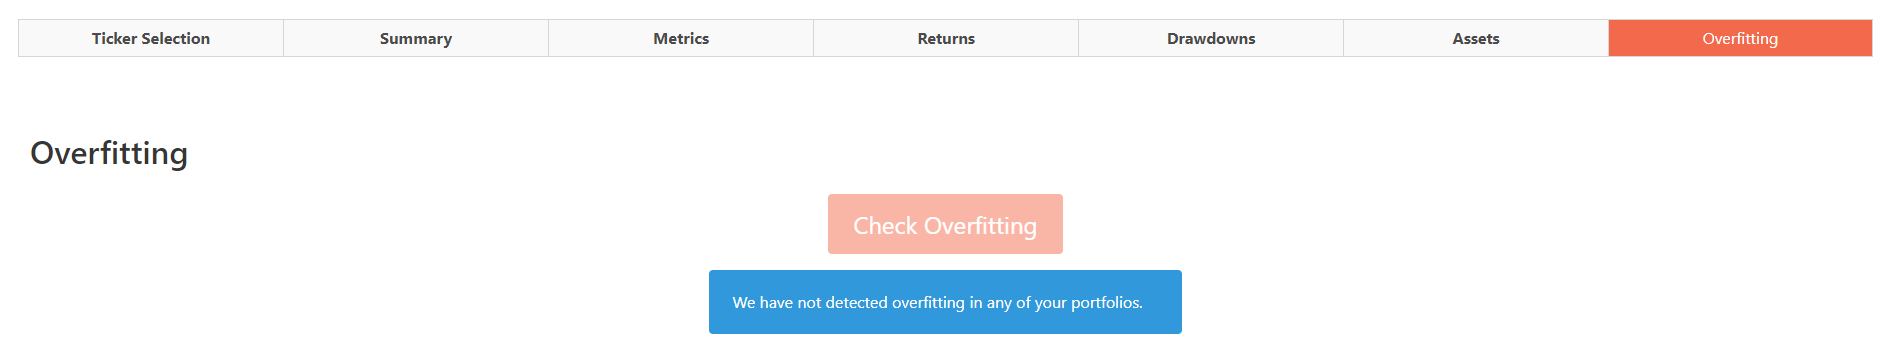
\includegraphics[width=\textwidth]{08Appendices/081User/081Pictures/overfitting.png}
   \caption{Overfitting Tab (source: http://thaliabacktest.xyz/dashboard/)}
   \label{overfitting}
\end{figure}

Alternatively, if the test detects overfitting, it will warn the user, highlighting the corresponding portfolio(s).

\end{document}
